%%%%%%%%%%%%%%%%%%%%%%%%%%%%%%%%%%%%%%%%%
% Masters/Doctoral Thesis
% LaTeX Template
% Version 2.4 (22/11/16)
%
% This template has been downloaded from:
% http://www.LaTeXTemplates.com
%
% Version 2.x major modifications by:
% Vel (vel@latextemplates.com)
%
% This template is based on a template by:
% Steve Gunn (http://users.ecs.soton.ac.uk/srg/softwaretools/document/templates/)
% Sunil Patel (http://www.sunilpatel.co.uk/thesis-template/)
%
% Template license:
% CC BY-NC-SA 3.0 (http://creativecommons.org/licenses/by-nc-sa/3.0/)
%
%%%%%%%%%%%%%%%%%%%%%%%%%%%%%%%%%%%%%%%%%

%----------------------------------------------------------------------------------------
%	PACKAGES AND OTHER DOCUMENT CONFIGURATIONS
%----------------------------------------------------------------------------------------

\documentclass[
11pt, % The default document font size, options: 10pt, 11pt, 12pt
%oneside, % Two side (alternating margins) for binding by default, uncomment to switch to one side
english, % ngerman for German
singlespacing, % Single line spacing, alternatives: onehalfspacing or doublespacing
%draft, % Uncomment to enable draft mode (no pictures, no links, overfull hboxes indicated)
%nolistspacing, % If the document is onehalfspacing or doublespacing, uncomment this to set spacing in lists to single
%liststotoc, % Uncomment to add the list of figures/tables/etc to the table of contents
%toctotoc, % Uncomment to add the main table of contents to the table of contents
parskip, % Uncomment to add space between paragraphs
%nohyperref, % Uncomment to not load the hyperref package
headsepline, % Uncomment to get a line under the header
chapterinoneline, % Uncomment to place the chapter title next to the number on one line
%consistentlayout, % Uncomment to change the layout of the declaration, abstract and acknowledgements pages to match the default layout
]{MastersDoctoralThesis} % The class file specifying the document structure

\usepackage{listings}
\usepackage{LatexExtensions/listings-golang} % import this package after listings
\usepackage{float}

\lstset{
  frame=top,
  basicstyle=\footnotesize,    % the size of the fonts that are used for the code
  tabsize=2,                              % tab size in blank spaces
  extendedchars=true,                     %
  breaklines=true,                        % sets automatic line breaking
  captionpos=b,                           % sets the caption-position to top
  mathescape=true,
  showspaces=false,           % Leerzeichen anzeigen ?
  showtabs=false,             % Tabs anzeigen ?
  xleftmargin=17pt,
  belowcaptionskip=1em,
  aboveskip=2em,
  framexleftmargin=17pt,
  framexrightmargin=17pt,
  framexbottommargin=5pt,
  framextopmargin=5pt,
  showstringspaces=false      % Leerzeichen in Strings anzeigen ?
 }


\DeclareCaptionFormat{listing}{\rule{\dimexpr\textwidth+17pt\relax}{0.4pt}\par\vskip1pt#1#2#3}
\captionsetup[lstlisting]{format=listing,singlelinecheck=false, margin=0pt, font={sf},labelsep=space,labelfont=bf}

\DeclareMathVersion{sans}
\SetSymbolFont{operators}{sans}{OT1}{cmbr}{m}{n}
\SetSymbolFont{letters}  {sans}{OML}{cmbrm}{m}{it}
\SetSymbolFont{symbols}  {sans}{OMS}{cmbrs}{m}{n}




\usepackage[utf8]{inputenc} % Required for inputting international characters
\usepackage[T1]{fontenc} % Output font encoding for international characters

% \usepackage{graphicx}
% \graphicspath{ {Figures/} }

\usepackage{palatino} % Use the Palatino font by default

\usepackage[backend=bibtex,natbib=true]{biblatex} % Use the bibtex backend with the authoryear citation style (which resembles APA)

\addbibresource{example.bib} % The filename of the bibliography

\usepackage[autostyle=true]{csquotes} % Required to generate language-dependent quotes in the bibliography

%----------------------------------------------------------------------------------------
%	MARGIN SETTINGS
%----------------------------------------------------------------------------------------

\geometry{
	paper=a4paper, % Change to letterpaper for US letter
	inner=2.5cm, % Inner margin
	outer=3.8cm, % Outer margin
	bindingoffset=.5cm, % Binding offset
	top=1.5cm, % Top margin
	bottom=1.5cm, % Bottom margin
	%showframe, % Uncomment to show how the type block is set on the page
}

%----------------------------------------------------------------------------------------
%	THESIS INFORMATION
%----------------------------------------------------------------------------------------

\thesistitle{Big Data Analytics on Container-Orchestrated Systems} % Your thesis title, this is used in the title and abstract, print it elsewhere with \ttitle
\supervisor{Kenneth M. Anderson} % Your supervisor's name, this is used in the title page, print it elsewhere with \supname
\examiner{} % Your examiner's name, this is not currently used anywhere in the template, print it elsewhere with \examname
\degree{Bachelor's degree in Informatics Engineering} % Your degree name, this is used in the title page and abstract, print it elsewhere with \degreename
\author{Gerard Casas Saez} % Your name, this is used in the title page and abstract, print it elsewhere with \authorname
\addresses{} % Your address, this is not currently used anywhere in the template, print it elsewhere with \addressname

\subject{Informatics Engineering} % Your subject area, this is not currently used anywhere in the template, print it elsewhere with \subjectname
\keywords{} % Keywords for your thesis, this is not currently used anywhere in the template, print it elsewhere with \keywordnames
\university{\href{http://colorado.edu/}{University of Colorado Boulder}} % Your university's name and URL, this is used in the title page and abstract, print it elsewhere with \univname
\faculty{\href{http://www.colorado.edu/engineering/}{College of Engineering and Applied Science}} % Your faculty's name and URL, this is used in the title page and abstract, print it elsewhere with \facname
\department{\href{http://www.colorado.edu/cs/}{Department of Computer Science}} % Your department's name and URL, this is used in the title page and abstract, print it elsewhere with \deptname
\group{\href{http://epic.cs.colorado.edu/}{Project EPIC Research Group}} % Your research group's name and URL, this is used in the title page, print it elsewhere with \groupname


\AtBeginDocument{
\hypersetup{pdftitle=\ttitle} % Set the PDF's title to your title
\hypersetup{pdfauthor=\authorname} % Set the PDF's author to your name
\hypersetup{pdfkeywords=\keywordnames} % Set the PDF's keywords to your keywords
\hypersetup{linkcolor=black}
}

\hyphenation{con-tain-er-ization orch-es-tra-tion orch-es-trated a-dop-ted}

\begin{document}

\frontmatter % Use roman page numbering style (i, ii, iii, iv...) for the pre-content pages

\pagestyle{plain} % Default to the plain heading style until the thesis style is called for the body content

%----------------------------------------------------------------------------------------
%	TITLE PAGE
%----------------------------------------------------------------------------------------

\begin{titlepage}
\begin{center}

\vspace*{.06\textheight}
{\scshape\LARGE \univname\par}\vspace{1.5cm} % University name
\textsc{\Large Bachelor thesis}\\[0.5cm] % Thesis type

\HRule \\[0.4cm] % Horizontal line
{\huge \bfseries \ttitle\par}\vspace{0.4cm} % Thesis title
\HRule \\[1.5cm] % Horizontal line

\begin{minipage}[t]{0.4\textwidth}
\begin{flushleft} \large
\emph{Author:}\\
\authorname % Author name - remove the \href bracket to remove the link
\end{flushleft}
\end{minipage}
\begin{minipage}[t]{0.4\textwidth}
\begin{flushright} \large
\emph{Supervisor:} \\
\supname % Supervisor name - remove the \href bracket to remove the link
\end{flushright}
\end{minipage}\\[3cm]

\vfill

\large \textit{A thesis submitted in fulfillment of the requirements\\ for \degreename}\\[0.3cm] % University requirement text
\textit{in}\\[0.4cm]
\href{https://fib.upc.edu}{Facultat d'Informàtica de Barcelona}\\\href{https://upc.edu}{Universitat Politècnica de Catalunya}\\[2cm] % Research group name and department name

\vfill

{\large \today}\\[4cm] % Date
%\includegraphics{Logo} % University/department logo - uncomment to place it

\vfill
\end{center}
\end{titlepage}

%----------------------------------------------------------------------------------------
%	DECLARATION PAGE
%----------------------------------------------------------------------------------------

% \begin{declaration}
% \addchaptertocentry{\authorshipname} % Add the declaration to the table of contents
% \noindent I, \authorname, declare that this thesis titled, \enquote{\ttitle} and the work presented in it are my own. I confirm that:

% \begin{itemize}
% \item This work was done wholly or mainly while in candidature for a research degree at this University.
% \item Where any part of this thesis has previously been submitted for a degree or any other qualification at this University or any other institution, this has been clearly stated.
% \item Where I have consulted the published work of others, this is always clearly attributed.
% \item Where I have quoted from the work of others, the source is always given. With the exception of such quotations, this thesis is entirely my own work.
% \item I have acknowledged all main sources of help.
% \item Where the thesis is based on work done by myself jointly with others, I have made clear exactly what was done by others and what I have contributed myself.\\
% \end{itemize}

% \noindent Signed:\\
% \rule[0.5em]{25em}{0.5pt} % This prints a line for the signature

% \noindent Date:\\
% \rule[0.5em]{25em}{0.5pt} % This prints a line to write the date
% \end{declaration}

% \cleardoublepage

%----------------------------------------------------------------------------------------
%	QUOTATION PAGE
%----------------------------------------------------------------------------------------

% \vspace*{0.2\textheight}

% \noindent\enquote{\itshape Thanks to my solid academic training, today I can write hundreds of words on virtually any topic without possessing a shred of information, which is how I got a good job in journalism.}\bigbreak

% \hfill Dave Barry

%----------------------------------------------------------------------------------------
%	ABSTRACT PAGE
%----------------------------------------------------------------------------------------

\begin{abstract}
\addchaptertocentry{\abstractname} % Add the abstract to the table of contents
Container-orchestration systems offer new possibilites to software architects seeking to make their software systems more scalable and reliable. In the past, these systems have been used to implement transactional software systems but, more recently, they have been applied to other areas including big data analytics. To understand the advantages and limitations such systems impose on software architects, I migrated an existing big data analytics infrastructure from a software architecture that required lots of work from its developers to deploy and maintain to the new software architecture provided by container-orchestration systems. My results show that scalability is increased, maintenance costs are reduced, and reliability is easier to achieve.
\end{abstract}

%----------------------------------------------------------------------------------------
%	ACKNOWLEDGEMENTS
%----------------------------------------------------------------------------------------

% \begin{acknowledgements}
% \addchaptertocentry{\acknowledgementname} % Add the acknowledgements to the table of contents
% I \ldots
% \end{acknowledgements}

%----------------------------------------------------------------------------------------
%	LIST OF CONTENTS/FIGURES/TABLES PAGES
%----------------------------------------------------------------------------------------

{
	\hypersetup{hidelinks}
	\tableofcontents % Prints the main table of contents

	\listoffigures % Prints the list of figures

	% \listoftables % Prints the list of tables

	\lstlistoflistings
}
%----------------------------------------------------------------------------------------
%	ABBREVIATIONS
%----------------------------------------------------------------------------------------

% \begin{abbreviations}{ll} % Include a list of abbreviations (a table of two columns)

% \textbf{LAH} & \textbf{L}ist \textbf{A}bbreviations \textbf{H}ere\\
% \textbf{WSF} & \textbf{W}hat (it) \textbf{S}tands \textbf{F}or\\

% \end{abbreviations}

%----------------------------------------------------------------------------------------
%	PHYSICAL CONSTANTS/OTHER DEFINITIONS
%----------------------------------------------------------------------------------------

% \begin{constants}{lr@{${}={}$}l} % The list of physical constants is a three column table

% % The \SI{}{} command is provided by the siunitx package, see its documentation for instructions on how to use it

% Speed of Light & $c_{0}$ & \SI{2.99792458e8}{\meter\per\second} (exact)\\
% %Constant Name & $Symbol$ & $Constant Value$ with units\\

% \end{constants}

%----------------------------------------------------------------------------------------
%	SYMBOLS
%----------------------------------------------------------------------------------------

% \begin{symbols}{lll} % Include a list of Symbols (a three column table)

% $a$ & distance & \si{\meter} \\
% $P$ & power & \si{\watt} (\si{\joule\per\second}) \\
% %Symbol & Name & Unit \\

% \addlinespace % Gap to separate the Roman symbols from the Greek

% $\omega$ & angular frequency & \si{\radian} \\

% \end{symbols}

%----------------------------------------------------------------------------------------
%	DEDICATION
%----------------------------------------------------------------------------------------

% \dedicatory{For my family and all their encouragement and support to travel to Boulder for this thesis}

%----------------------------------------------------------------------------------------
%	THESIS CONTENT - CHAPTERS
%----------------------------------------------------------------------------------------

\mainmatter % Begin numeric (1,2,3...) page numbering

\pagestyle{thesis} % Return the page headers back to the "thesis" style

% Include the chapters of the thesis as separate files from the Chapters folder
% Uncomment the lines as you write the chapters

% Chapter Template

\chapter{Introduction} % Main chapter title

\label{Chapter1} % Change X to a consecutive number; for referencing this chapter elsewhere, use \ref{ChapterX}

Big Data Analytics is a research area undergoing intense interest and rapid development. Data is being generated by sensors and computing systems at an ever increasing rate. Indeed, it is estimated that every month, seventy-two petabytes of information are moved around the Internet.\parencite{ciscoreport} This amount is expected to grow to 232 petabytes/month by 2021.\parencite{ciscoreport} This rapid growth is a significant challenge to the designers of software systems and to the field of computer science in general. New software infrastructure will need to be designed to support this demand and to extract useful information from it. In addition, a wide range of techniques and technologies must be mastered to keep analysis time low at this scale. 

Containerization is one technique that can be useful in addressing these challenges and tools/technologies that provide containerization services are seeing increasing interest and development as well. The ability to run software in separate environments has been a revolution for the tech industry. Containerization is an abstraction for avoiding long installation processes on each system a software development team needs to run their software. It is similar to virtual machines but optimized to use system resources instead of simulated resources. Put another way, a virtual machine image contains everything needed to simulate a separate operating system. If you have multiple copies of that image, each image contains a complete copy of the operating system and all other components needed to run your software, wasting valuable disk space and consuming extra memory at run-time. With containerization, each container image contains just the software that you want to deploy and its required packages and the containerization run-time system provides a unified operating system for running all containers. Thanks to companies like Docker,\footnote{\href{https://docker.com}{https://docker.com}} containers are becoming a de facto standard for software development and deployment. Its ease of use and consistent behaviour between machines makes it an attractive option for developers.

However, there are a few complexities: network configuration, interaction between containers, system updates, and more. To solve these complexities, container-orchestration systems were developed. These systems provide another abstraction layer on top of containers,  taking over the management of an underlying containerization technology. In particular, the container-orchestration system is in charge of coordinating containers, creating them, destroying them, etc. The entire container life cycle is controlled by the orchestration system.

As these orchestration systems become more popular, software architects must create new software architectures that embrace the new possibilities that these systems provide. Some features that previously were difficult to achieve are now available to any software architect. Applications no longer need to have a static infrastructure; container-orchestrated systems can grow and decrease system resources on demand. Systems can be split into small microservices and deployed across a cluster of machines; there is no need to merge system components into a big monolithic application anymore.

Furthermore, cloud providers are adding support for container-orchestrated systems, making it even easier to deploy complex infrastructures. Due to the similarities between different cloud offerings, you can design this new style of software system independent of a specific provider. One benefit to container-orchestrated systems is that it provides a means for finding new ways to solve problems associated with making use of parallelism and scaling a software system to handle ever increasing amounts of data. If properly designed, surges in demand can be met by spinning up additional copies of core system services balanced across the cluster of machines you have reserved from your cloud provider.

The goal of my thesis is to explore how this new style of software architecture can be used to deploy software infrastructures that are used to perform big data analytics. In particular, I will be migrating an existing big data infrastructure to make use of the techniques and technologies offered by container-orchestrated systems and compare the new version of the system with its previous incarnation along a number of dimensions. 

% Chapter Template

\chapter{Background} % Main chapter title

\label{Chapter2} % Change X to a consecutive number; for referencing this chapter elsewhere, use \ref{ChapterX}

%----------------------------------------------------------------------------------------
%	SECTION 1
%----------------------------------------------------------------------------------------

Before digging into the project itself, we need to understand the problem area. 

\section{Project EPIC}

EPIC (Empowering the Public with Information in Crisis) is a project at the University of Colorado Boulder. Its focused in crisis informatics, an area of study that examines how people use different technologies to interact during emergencies and their impact on emergency response. 
 
Project EPIC has a long history on software engineering. Since 2009, this project has done research on large data storage and analysis. When large amounts of data are being collected, software engineers need to focus on structuring this data so it’s easy to perform analysis . In addition, this data needs to be easily accessible for analysts.
 
The research group has with it’s own Big Data analytics system running. Developed over the past 8 years by different software engineers researchers, the mentioned system counts with 3 different parts Collect, Analyze and Analytics. EPIC Collect is the in-house Twitter Streaming client that works 24/7 retrieving tweets from the various events that need to be monitored in real time. Since 2009 this software has been collecting tweets with an uptime of 99\%. On the storage layer, we have Cassandra. This NoSQL database is focused on writes and allows a  really high input. On the other side we have EPIC Analyze, built to help analysts access the data that has been collected on Cassandra. Finally EPIC Analytics is a large machine where analysts execute intensive processes over the collected data.

\section{Containerization}

We understand containerization as operating-system-level virtualization. This technology allows program to be run inside a system, isolated  from each other and the host system. It works similarly than traditional virtual machines from the point of view of a program, but makes use of the underlying system resources instead of running a full powered operating system. It provides an abstraction to for programs to run in. 
 
There are many containerization platforms around, however the most used and the one we will use for this project is Docker. This platform was originated as an internal tool in a PaaS company and later on open-sourced. Thanks to many contributions from different companies, this project grew becoming the most used containerization software. It’s able to run on almost any system and has many integration. In addition, almost all container orchestrator systems support Docker containers


\section{Container orchestration technologies}

When containerisation technologies raised due to a migration to microservice architectures, big companies needed a way to manage their containers in a more friendly way. Interconnecting containers, managing their deployment, scaling easily, all this tasks were possible with containers, but they were really difficult. This is why container orchestrations systems were born. In order to manage container, the mentioned systems add an abstraction layer on top of the systems, making such tasks easier to perform.
 
There are a few available container orchestration systems available at the moment. The most popular ones are Kubernetes and Apache Mesos. In this project, we will further explore Kubernetes. The main reason for this is that thanks to its open source community it’s easier to find tutorials and courses. In addition, there are a lot of big companies that are backing this project and contributing to it, which provides a security of a long-term support.
 
Google Cloud seems like the best fit to host Kubernetes as it has a managed cluster option where we don’t need to worry to install and wire up the system. In addition, thanks to Google being part of the maintaining team for Kubernetes, there’s a great support for Google Cloud infrastructure on Kubernetes.


\section{Microservices architecture}


Microservices is an approach to distributed systems that promote the use of small services with specific responsibilities that collaborate between them, rather than big components with a lot of responsibilities that make interaction more difficult.
 
In addition, thanks to new technologies like containers and container orchestrated systems, they are quickly becoming a standard on the design of big software systems. This type of architecture has been adopted by many companies as it provides a more maintainable model. 
 
Another of the key advantages of Microservices is that it makes it easier to adopt different technologies for each component. In addition to containerization it decouples differents parts of a system systems. This allows a better optimization of technology depending on the feature that each microservice needs to offer. For example a microservice that needs to store a highly related data can make use of separate graph database, exposing a REST API, allowing for a completly abstraction. At the same time a microservice that needs to store big documents can use a document store database underneath, allowing for a better optimization. 
 
 
 
Having small microservices do specific tasks, makes development cycles faster and more independent. Making incremental deployment way easier and less dangerous. They also make it easier to scale systems. We could individually scale parts of the system independently depending on their usage.
 
Microservices avoid falling in the same problems that previous service-centered architectures had, by centering on their architecture and letting the architect decide the messaging system or deployment type.
 
In addition microservice architecture allows for a better reliance, as each microservice is independent, if one fails, the rest can remain unaffected. This finds a perfect match with container orchestration systems, as they can abstract health checks on microservice as well deploy again microservices that failed.
 
In terms of designing microservice architectures there are a couple of approaches that are equally used at the moment: coreography and orchestration\parencite{microservices}.

%-----------------------------------
%	SUBSECTION 1
%-----------------------------------
\subsection{Coreography}

Coreography approach centers all interaction on a publish-subscribe philsophy. Events are propagated through the system in an asyncronous basis. When something happens in a microservice, it gets published into a public queue. Other microservices can subscribe to this queue and act consequently when they receive an event.
 
This approach makes it the system more flexible, removing the responsability of knowing who to send messages to from the microservices. We can add more components easily without having to modify the existing ones. 
 
However, we need extra components in order to make sure that all tasks are performed once an event is published. We can acomplish this by installing and mantaining a monitoring solution.

%-----------------------------------
%	SUBSECTION 2
%-----------------------------------

\subsection{Orchestration}

Orchestration centers interactions in request/response iteractions. Each microservice requests information to any other microservice. For this approach we need of a proper service discover backend. In addition if the service is down, we need to make sure that each microservice retries and is capable of failing gently. 
 
The good thing is that we would be sure that all actions are performed by the end of an action. However if a components takes too long to answer we could break the entire action.
 
A more modern approach to orchestration has been developed with Service meshes. This components take the responsibility of balancing requests as well as allowing for service discovery to happen, they avoid bad crashes by retrying requests. They work by adding a sidecar to all microservices acting as proxy between the microservice and the outside network. Together with a manager that controls service discovery, load balancing and retrying counters. However these are still new technologies being developed and are still on their early releases. In addition they don’t include the choreography extensibility capabilities.


%----------------------------------------------------------------------------------------
%	SECTION 2
%----------------------------------------------------------------------------------------

\section{Messaging systems}

Messaging systems organize queues of messages produced by some microservices and notify subscribed systems that are consuming queues when they arrive. Their main objective is to  can decouple components and to have a cache if the consumers can’t digest all the incoming messages. This allows for more reliable systems as system don’t depend on the mutual availability to pass messages as they would if they had to use other messaging system like HTTP.
 
There are many options used nowadays the most popular being Apache Kafka and RabbitMQ. Kafka, is a decentralized, high availability system that allows us to publish messages organized by topics. It allows for high parallelizability thanks to the partitions on topics, which lets you read and write at a higher rate in a parallel way.  Each partition can have one consumer associated to it, which makes it faster to read. 
 
Another good thing about Kafka is its persistence system. Thanks to a great integration with the kernel, it performs and persists data faster than other systems. This is due the fact that gives the responsibility to flush to disk to the kernel, taking advantage to disk page caching and memory caching implemented into current operating systems.
 
In addition, Kafka it’s one of the most used messaging systems in the industry nowadays. Many companies use it on their production systems to decouple their systems and increase code responsability repartition. In addition it has a really strong community behind it, as well as some major technology companies like Linkedin maintaining it. Other messaging options include RabbitMQ or NATS.
 
Messaging systems are needed for choreography microservice architectures, as they are the communication layer between microservices. 


\section{Big Data storage systems}

We will be tracking Twitter with the Streaming API. As the API is limited to provide a 10\% of the total tweets generated in twitter every minute, we can estimate how many tweets will go through our system. Last report available of tweets per seconds is from 2013. The rate was 5700 tweets\parencite{tweetsRecord} per second on average.  Which means that our system should be able to store 570 tweets every second. In addition we need a platform that scales well with our increasingly large datasets. As previously studied in the EPIC project\parencite{mySQLnoSQL},  we would need to use a NoSQL database instead of a relational database to support the high throughput of tweets and make the system more scalable.

 
On the other hand we also need a system that allows analytical and operational queries happening at the same time. We would like to be able to analyze our data in real time without having to stop its storage. Given that some analysis may take a few minutes due to the high amount of items to analyze, we need to  have a system that allows a high throughput for both parts. In this case Cassandra is the best option as the number of operations per seconds scales the most compared to other NoSQL alternatives, especially with operational and analytical workloads\parencite{benchmarkNoSQL}.
 
To store tweets we base our table structure on the current EPIC Analyze structured data storage in Cassandra as we can see on the CQL in the next page. In addition we also add an index on the event\_name attribute so that we can access per event faster. We need to add the index as a lot of queries are performed per event, and so we would benefit from accessing tweets from each event in the fastest way.


\begin{lstlisting}[language=SQL, caption={Tweets CQL table script}, float, floatplacement=H ]
CREATE TABLE twitter_analytics.tweet (
    id uuid,
    t_id text,
    event_kw text,
    event_name text,
    hashtags list<text>,
    media_url text,
    t_coordinates text,
    t_created_at timestamp,
    t_favorite_count int,
    t_favorited boolean,
    t_geo text,
    t_is_a_retweet boolean,
    t_lang text,
    t_retweet_count int,
    t_retweeted boolean,
    t_text text,
    u_created_at timestamp,
    u_description text,
    u_favourites_count int,
    u_followers_count int,
    u_friends_count int,
    u_geo_enabled boolean,
    u_id text,
    u_lang text,
    u_listed_count int,
    u_location text,
    u_name text,
    u_screen_name text,
    u_statuses_count int,
    u_time_zone text,
    u_url text,
    u_utc_offset int,
    um_id text,
    um_name text,
    um_screen_name text,
    urls list<text>,
    PRIMARY KEY (id, t_id))
\end{lstlisting}


\section{Software development in microservices architectures}
Thanks to container-orchestrated systems and the popularization of container systems, software development is easier. With microservices, focus moves out of one component software architecture to organizing the whole system. Now, we can focus on packaging alone components instead of having to packaging all of them at once, which makes the development more flexible. This would allow for a more continuous development in the system allowing for a better performance optimization, and an easier way to keep the system updated with the last set of technologies.

% Chapter Template

\chapter{Problem Statement} % Main chapter title

\label{Chapter3} % Change X to a consecutive number; for referencing this chapter elsewhere, use \ref{ChapterX}

The goal of my thesis is to explore the benefits and limitations in using container-orchestration systems to build and deploy software systems that engage in big data analytics. To perform this exploration, I will be redesigning the Project EPIC software infrastructure as a set of microservices---each inside a separate Docker container---that are deployed on a cluster of cloud-based machines via a container-orchestration system. The current infrastructure was manually deployed on a set of physical machines in a local data center and was not developed using microservices or containerization. My hypothesis is that I’ll be able to achieve greater scalability and reliability with the new architecture with significantly reduced maintenance costs. I will also explore whether I am able to achieve greater query flexibility and overall performance using this new style of software infrastructure. My specific research questions are:

\begin{enumerate}
	\item What advantages and/or limitations will the new Project EPIC infrastructure have with respect to its predecessor?
	\begin{enumerate}
		\item Is it more reliable? If so, why?
		\item Is it more scalable? If so, why?
	\end{enumerate}
	\item Does the new infrastructure have lower maintenance costs than the existing infrastructure?
	\begin{enumerate}
		\item Is it easier to deploy?
		\item Is it easier to upgrade?
		\item Is it more resilient to failures? If so, how?
	\end{enumerate}
\end{enumerate}



 % Chapter Template

\chapter{Evaluation} % Main chapter title

\label{Chapter4} % Change X to a consecutive number; for referencing this chapter elsewhere, use \ref{ChapterX}

In order to evaluate this project we are going to compare the proposed architecture with the existing EPIC architecture in reliability and scalability as well as performance and real time delivery as proposed in the problem statement. We will also evaluate manteinability and future software development.

\section{Reliability}

To analyze reliability between systems we will analyze how well each system recovers if a components fails. We are interested to see how much time does it take to have the system recover if something failed. In addition we want to check what mechanisms do we have in both cases to check the health of each component. This would be useful to restart parts that have stopped working. 

\subsection{Current infrastructure}

Reliability on the existing EPIC infrastructure needs to be studied separately between EPIC Collect and EPIC Analyze. Collect is designed to be highly available. Using different techniques like cron jobs  that check the state and other. EPIC Collect is a really reliable system. It has been available 99\% of the time since 2012, making it really reliable for analysts to trust that their tweets are being collected. In the worst case scenario, EPIC Collect takes X seconds to recover. This is due the fact that the cron job that checks that EPIC Collect is running is scheduled every 5 seconds.

EPIC Analyze doesn’t have the same availability. The system has suffered multiples upgrades and depends on different pieces that can fail. Analyze depends on a separated Cassandra with Solr as well as a Redis cluster. If any of those two were to fail, the system would go down, being completely unusable. There’s no automatic recovery procedure. 

In conclusion, the current EPIC infrastructure depends of what secure layers developers have added to their programs, which makes it hard to develop and costly to keep it reliable. In addition, the deployment of the system is manual, which could involve human errors on deployment that could cause future instability of the system. This could be caused because components overlap each other RAM usage causing a full node of the cluster to go down.

\subsection{Proposed infrastructure}

In this case, reliability is a responsibility from the container orchestrated system. In our case, Kubernetes includes a controller manager on the master node. This component of the cluster keeps track of the status of each one of the containers running. The controller manager makes sure that a certain amount of replicas are up and running. If any container stops running at some point, the controller manager will make sure to schedule a new container and run it on an available node. This check is done on demand when there are new deployments requested or whenever a node notifies that a container is down.

 In addition to the controller manager, we also have the scheduler. This component makes sure that new container are scheduled in the best node possible. Kubernetes allows you to configure the amount of memory and cpu usage permitted by container, allowing the scheduler to find the best fit for each deployment request. 

Thanks to this deployment automation, node failures can be avoided easily as well as resources get a more optimized usage than if doing this process manually. Finally something else that Kubernetes allows to do natively is to rollout new versions of a service with no downtime. To do so the controller manager deploys the new version before removing the previous.  This is really useful for example in the Twitter tracker module, as this way all tweets get tracked even when the keywords change. In this case, the controller manager deploys a new version with the new keywords updated. Once it starts to run, it kills the previous version, which means that there’s always at least one version running and tracking all tweets. This ensures that we can get all tweets.

To test it, we left the system tracking for 11 days with no interaction from the user. As we can observe in Figure~\ref{fig:pods}, each instance has restarted many times. This could be caused when the  system reached peaks of load. With the limited amount of resources availables, Kubernetes has to kill some containers to avoid the whole system collapsing. Note that some instances say that have been existing for less than 2 days, this is due the fact that Kubernetes will restart the count if it needs to do a hard restart.



\begin{figure}
\centering
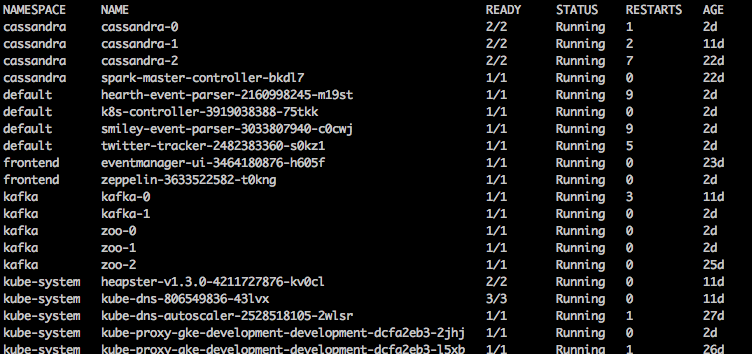
\includegraphics[width=\textwidth]{Figures/pods}
\decoRule
\caption[Status instances]{Status instances after 11 days}
\label{fig:pods}
\end{figure}

\section{Scalability}

We want a system that adapts to our needs, so we want a high scalability for it. We want to avoid wasting resources unnecessarily as well, so we want to be able to fit our available infrastructure. To analyze this we will see how easy is to scale each system and how scaling affects performance in either infrastructure.

\subsection{Current infrastructure}

The current infrastructure is not easy to scale. If we need to scale EPIC Collect, we would need to run manually a new instance, add cron jobs as well as add new Twitter credentials for it. This is one of the reason why EPIC Collect doesn’t do data normalization, if we added data normalization to the current EPIC Collect then on traffic spikes the system could be overloaded and would not be able to scale during high demand tweet incoming. 

Regarding storage, scalability is high thanks to Cassandra. Adding new nodes to the cluster it’s a pretty straight forward process. However regarding it will be difficult to add more Cassandra nodes than machines we have available, due to the fact that we will need to add more open ports to the outside of the machine. This is a small step back, as it’s not really complex. 

Regarding EPIC Analyze, the only thing we could scale, apart from storage, would be the frontend module. However that would mean adding a standalone load balancer in front of the service, which makes it a complex process if done manually and adds more complexity to maintain it. Also, we would need to add an external component to keep session information consistent across all the replicas, even though we could reuse the current Redis cluster to do so. The application would still need a refactor either way. 

In conclusion, it’s not really easy to scale the current infrastructure.

\subsection{Proposed infrastructure}

On the other side, the proposed architecture has a better and easy way to scale thanks to Kubernetes.

When deploying a service we can specify how many replicas we want to deploy. The controller manager will try to schedule as many replicas as it has been specified if there are enough resources. In addition, we tried to approach the design of the different components in a stateless way so that deploying new replicas would not require any additional change in the components. To achieve this, we moved the state to the infrastructure. The components are unaware of the state of the system, which makes it easy to add replicas. When added they do their task independently.

We could  also easily automate scalability  for each component depending on their CPU usage. If a certain container is in 90\% of their CPU usage, we can make that the system increments the number of replicas. This way the underlying resources can be administered in regards of the current needs of the system.

In terms of time to scale, it’s a matter to send the changes to Kubernetes. This can be done with a single command thanks to the command line tool kubectl or using the web interface for Kubernetes. Scaling is an integrated tool into container orchestrated systems, specially Kubernetes.

\section{Performance}

In order to analyze performance between both systems we need to take into account resources availables. All the analysis has been performed in the previously deployed 4 node cluster, each one with 4Gb or RAM and 1 virtual CPU. We will measure time to execute a word count script for a  certain number of collected tweets. We chose word count as it’s a highly a parallelizable program. 

Regarding performance we need to take into account different aspects. The current EPIC architecture performs really well when asking for some very specific queries. However, if we want more general queries or complex ones we would have to download the dataset to work with it with local tools, which makes analysis way slower. 

The goal for the architecture should be to give tools for analysts to develop their work without having to wonder how it was implemented. For this reason I focused on delivering a query flexible system that let’s query data in different ways. 

In order to analyze the performance in an overall way, we will take an example of dataset collected in the current infrastructure and one in a WordCount exercise. I selected WordCount as it’s a simple to describe data analysis and it has a high degree of parallelization. This way we can see how each system takes advantages of the distributed system.

In the new infrastructure we can use Spark running on top of Cassandra. This work should be optimized thanks to having a spark worker on each cassandra node, minimizing all network traffic by using data locality. 


\begin{lstlisting}[language=scala, caption={WordCount Spark script},float, floatplacement=H]
val table = sc.cassandraTable("twitter_analytics", "tweet")
val words = table.select("t_text").flatMap(l => l.getString("t_text").split(" "))
      .map(word => (word.toLowerCase,1)).reduceByKey(_ + _).map(_.swap).sortByKey(false,1)
\end{lstlisting}



To check how the query is performed we will look into the debug string from Spark. This is string is used to check how Spark will execute a query into its cluster. Each indentation is a map stage, and each + is a shuffle phase. As we can see in Listing~\ref{lst:rddebug}, Spark is not doing any shuffles until the reduce stage, meaning that it’s optimizing the query to take advantage of data locality by executing maps on the same node that the data is loaded to.



\begin{lstlisting}[language=scala, caption={Debug string rdd}, float, floatplacement=H, label={lst:rddebug}]
(1) ShuffledRDD[112] at sortByKey at <console>:31 []
+-(176) MapPartitionsRDD[111] at map at <console>:31 []
    |   ShuffledRDD[110] at reduceByKey at <console>:31 []
    +-(176) MapPartitionsRDD[109] at map at <console>:31 []
        |   MapPartitionsRDD[108] at flatMap at <console>:31 []
        |   CassandraTableScanRDD[107] at RDD at CassandraRDD.scala:15 []
\end{lstlisting}


As we can see in Figure~\ref{fig:wordcountplot} the Word Count script performance is not linear, but it performs better with a bigger amount of tweets to analyze. This could be due the fact that the bigger value is being accessed as a total, therefore avoiding accessing indexes. This would make it quicker. We would need more results in order to analyze if this is true or not. However due to a timeout on reaad access to disk this can’t be performed. This is caused due to having really big indexes and big partitions on Cassandra. 

\begin{figure}
\centering
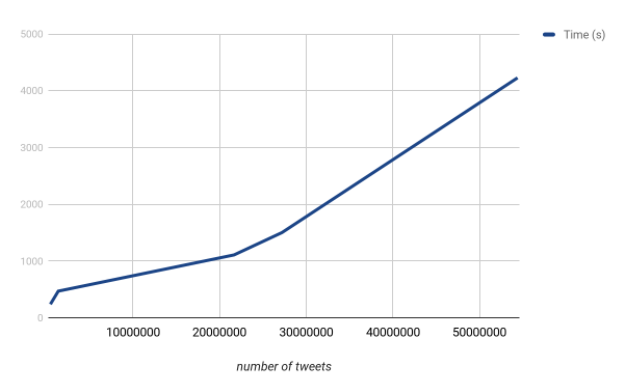
\includegraphics[width=\textwidth]{Figures/wordcountplot}
\decoRule
\caption[Wordcount time plot]{Plot on wordcount time for dataset size}
\label{fig:wordcountplot}
\end{figure}

To solve this tradeoff, we could move the index to primary key, adding an incrementing partition key to balance distribution between nodes similarly as random key. This is inspired to the column family distribution proposed in the work by Ahmet Arif, but using structured rows for each tweet instead of multiple JSON objects on each column. However due to the work being more focused on the container infrastructure part and concept development, this could not be performed during this thesis work.

On the other side, the current EPIC infrastructure is mainly oriented to collect tweets. Analysis are performed in dedicated machines that have a high number of cores and high RAM memory. In EPIC, mainly most of this analysis are performed in EPIC Analytics. However we need to take into account that due to the structure of the current system, batch analytics are performed after data has been extracted from Cassandra and therefore we can’t fully compare both system in terms of time to obtain a result since tweet collection. The current EPIC infrastructure is prepared to answer queries extracting data and running batch analysis. 

\begin{table}
\centering
\begin{tabular}{l l}
\toprule
\textbf{Number of tweets} & \textbf{Time (s)} \\
\midrule
490199 & 238 \\
1400884 & 469 \\
21680851 & 1107 \\
27199614 & 1500 \\
54395957 & 4228 \\
\bottomrule\\
\end{tabular}

\caption{Number of tweets in dataset vs seconds took to perform word count}
\label{tab:numtweets}
\end{table}

To solve this tradeoff, we could move the index to primary key, adding an incrementing partition key to balance distribution between nodes similarly as random key. This is inspired to the column family distribution proposed in the work by Ahmet Arif\parencite{batchreal}, but using structured rows for each tweet instead of multiple JSON objects on each column. However due to the work being more focused on the container infrastructure part and concept development, this could not be performed during this thesis work.

On the other side, the current EPIC infrastructure is mainly oriented to collect tweets. Analysis are performed in dedicated machines that have a high number of cores and high RAM memory. In EPIC, mainly most of this analysis are performed in EPIC Analytics. However we need to take into account that due to the structure of the current system, batch analytics are performed after data has been extracted from Cassandra and therefore we can’t fully compare both system in terms of time to obtain a result since tweet collection. The current EPIC infrastructure is prepared to answer queries extracting data and running batch analysis. 


\section{Real time analytics}

Real-time analysis has been approached before in the Project EPIC\parencite{batchreal}. However the previously mentioned approaches have a limited number of queries that can be answered in real time. Adding new queries would mean having to refactor the code and deploy again. The data used would also start to be collected once it’s deployed. Even though this approach gives result in a really low time, it lacks flexibility when it comes to custom queries. If analysts want custom queries, they would have to download the datasets and run their own custom analysis. This approach can be difficult, we need to predict what are the queries that we will need to answer ahead of time and sometimes this can be close to impossible.

For the new system, we took a more flexible approach. In order to increase flexibility, we sacrifice response time. Queries can be run on Spark while data is being collected, which makes their results near-real-time. We have a delay between when we start the query and when it ends, meaning that new data may have arrived during the query execution may have not been taken into account. 

This approach may seem as a lost in performance. However if analysts need custom analysis, this approach grants them a faster option. In addition, we allow for the analyst to run the query in an already existing system, which allows for the analysts to avoid having to configure their own system. Finally, thanks to the system decoupled architecture, it is possible in the future to add some real-time analysis by adding new consumers in the raw\_tweets queue that perform the mentioned static analysis, allowing for the existing feature in the current system to be re-deployed back in the new system.

\section{Software development and maintenance}

One of our goals was to develop a system that was easier to maintain. That was one of the reasons to adapt microservices was to avoid having components get outdated by making it easier for developers to onboard on the code and maintain it. In addition we also want to compare how easy would be to replace a component and code it from the ground up.

\subsection{Current infrastructure}

Currently the code is divided in 2 big monoliths. This can be a disadvantage on terms that developers must dig into the code of at least one of them in order to perform maintenance. This can be an small overhead as both of the projects are quite big. 

EPIC Analyze has 5086 lines of code. On boarding this part can be difficult. Specially since it uses a pretty closed framework as Ruby on Rails is. This can be a difficulty in terms of having to write new code, anyone who wants to write something need to learn the usage of Ruby on Rails. This framework is big and has a quite fast learning curve. However, it can be difficult as it implements practices that sometimes are not obvious for a developer coming from other frameworks. In addition to the code, we have a slow deployment process. In order to update the deployed version of EPIC Analyze, we need to restart the server manually. This makes it difficult to deploy, which in result turns into a really slow development process. Development for Analyze happens on a git repository, this makes collaboration easier between different developers.

EPIC Collect is difficult to analyze as it’s not on a git repository. Written in Java it’s built thinking on efficiency first.  This can be a bit of a difficulty in terms of collaborating and maintaining the code. In addition deploying new versions involves a lot of effort as it doesn’t only involve deploying the code, but also maintain the Tomcat server. We also need to take into account all the processes that are keeping EPIC Collect alive. Due to the fact that this scripts are embedded onto the development of EPIC Collect, we need to redeploy them manually.

\subsection{Proposed infrastructure}

The proposed infrastructure is divided into multiple different pieces. On one side we have the components code, divided between Python and Go code. On the other side we have the declaratives documents on YAML that specify how to deploy the infrastructure into Kubernetes.

\begin{itemize}
	\item \textit{Twitter tracker (Go)}: 108 lines 
	\item \textit{Kubernetes controller (Python)}: 145 lines
	\item \textit{Event manager UI (Python/Django)}: 2090 lines
	\item \textit{Tweet normalizer (Python)}: 209 lines
\end{itemize}

Code is more equilibrated distributed between different parts. The good thing is that we are not tied into an specific and unique framework. Making code small makes it easier for other developers to understand the purpose of each component. In addition thanks to separating responsibilities into microservices we can make collaboration easier by letting different developers work on different parts without crossing each other.

Something that also helps is that we can use different technologies in each component. This means that we can focus on building on the best available option for what we need to do. It also allows for a better pivoting of a component into a language that the maintainer prefers. If it can be containerized then it doesn’t matter what language or technology stack we use. It will be easily deployed into Kubernetes.

Finally we have the YAML files that store how the Kubernetes system looks like. All the system is declared in 3345 lines. There are many tools being released that will help make this code smaller. However right now the best option is to manually write and review each component in Kubernetes YAML files.



% Chapter Template

\chapter{Implementation} % Main chapter title

\label{Chapter5} % Change X to a consecutive number; for referencing this chapter elsewhere, use \ref{ChapterX}

In this section, I provide implementation-related details of my software prototype. The prototype is fully implemented and running on a set of nodes hosted by Google Cloud. We created four nodes in total each with one virtual CPU and 4 gigabytes of RAM. On those nodes that host Cassandra, we reserve 1 gigabyte of RAM for Cassandra’s exclusive use and allow the remaining memory to be used by other components deployed on those nodes (such as Apache Spark). The nodes that host Cassandra are deployed using a feature from Kubernetes called stateful sets. This data structure associates persistent volumes with particular system components such that data is preserved across restarts and crashes. They are designed to be used with distributed databases like Cassandra making it easy to add and remove nodes that host Cassandra at run-time. Thus, if we add a new node to our Cassandra cluster, Kubernetes ensures that a new persistent volume is created and attached to that node and then ensures that each time that node is activated the same persistent volume is made available to the database running on that node.

As mentioned above, we also designed our Kubernetes configuration to deploy an instance of an Apache Spark worker on each Cassandra node and then also specified one additional node to serve as the Apache Spark master node. A container with Zeppelin was also deployed configured to send queries to the Spark master node via Zeppelin’s cassandra-spark library.

I now present details on how each of the custom components discussed in Chapter \ref{Chapter4} were implemented. In general, microservices were implemented first in python for ease of prototyping and then switched to a different implementation language if performance problems were detected. Furthermore, all microservices were placed in individual Docker containers which were then deployed via Kubernetes as dictated by the Infrastructure Manager. Further details on each component are now presented:


\begin{itemize}
	\item \textbf{Event Manager UI:} The event manager is implemented as a stateful django web application. It supports CRUD operations on events. Any change of state is pushed out as a message on a Kafka queue (and acted upon by the Infrastructure Controller). It stores its data in SQLite as a file on a Google Cloud persistent disk. This set-up ensures that it can find its state across restarts.
	\item \textbf{Infrastructure Controller:}  This controller is written in python and makes use of python libraries that allow it to interact with Kafka and Kubernetes. When it receives a message from the Event Manager UI, it issues commands to Kubernetes to declare the new state of the world. If an event is no longer active, its associated Tweet Normalizer will be shut down. If a new event is specified, a new instance of the Tweet Normalizer is configured and deployed.
	\item \textbf{Twitter Tracker:} The Twitter Tracker was first implemented in Python but I discovered that python’s run-time engine was not fast enough to handle consistently high streaming volumes over long periods of time. As a result, I reimplemented this microservice in Go for better reliability and performance. As discussed above, this service submits keywords to Twitter’s Streaming API and then stores each tweet that it receives in a Kafka topic. The infrastructure controller is the one in charge of deploying and updating the instance. A set of all the tracked keywords is passed as environment variable on start by Kubernetes To update the keywords Kubernetes perform a rolling update by creating a new instance and destroying the old one once the new one has correctly started the stream. 
	\item \textbf{Twitter Normalizer:} The Twitter Normalizer is the one component in my infrastructure that can be instantiated multiple times and needs to monitor a different set of keywords in each instance. To facilitate this, I had the Infrastructure Controller direct Kubernetes to pass the keywords needed by each instance of the Twitter Normalizer as environment variables. Kubernetes could then deploy an instance of the Twitter Normalizer Docker container onto a node, configure its environment variables to match the keywords of the given event, and launch the microservice. The Twitter Normalizer was implemented in Python but specific C-based libraries were used to implement tasks that it executes over and over, e.g. loading and parsing JSON objects. This technique enabled the Twitter Normalizer to process the incoming stream of tweets with acceptable performance.
\end{itemize}

\section{Deploying the System}

Deploying my prototype is straightforward given the use of Google Cloud and Kubernetes. As mentioned above, I created a four-node cluster with each node allocated 1 virtual CPU and 4 gigabytes of RAM. Kafka and Cassandra/Spark are deployed first. In my prototype, I created two Kafka brokers that work together to manage the two primary topics needed by my design (the queue between the event manager and the infrastructure controller and the queue between the Twitter tracker and all instances of the Twitter normalizer) and instances of Cassandra/Spark on three of our four nodes. We then deploy the containers for our two front-end components: Zeppelin and the event manager. Finally, we deploy an instance of the infrastructure controller. All other components will be deployed by the infrastructure controller (including the Twitter tracker) when it receives a message from the event manager. This approach makes sense since there is no need to have the Twitter tracker and the Twitter normalizers running if there are no events to collect.

\newpage
\section{Front-End Components}

Figure \ref{fig:eventmanager} shows the user interface of the event manager. Each event is shown in a separate box with information about the event’s keywords. There are controls for creating new events and a separate control for sending a message to the infrastructure controller with the most recent state of the world. Events can be edited/deleted by controls that appear when its box is selected. Figure \ref{fig:zeppelin} shows the user interface provided by Zeppelin. Queries can be submitted via a textbox and results can be displayed in tables or via bar graphs (as shown).

\begin{figure}
\centering
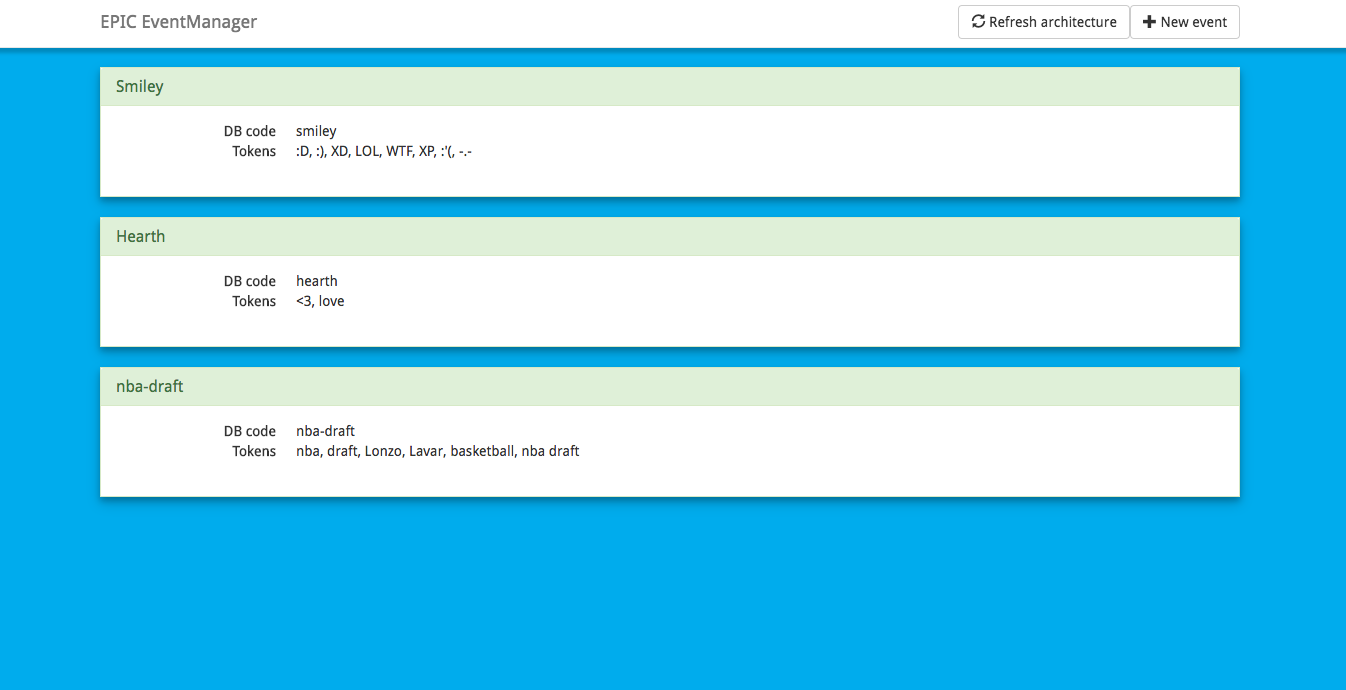
\includegraphics[width=\textwidth]{Figures/eventmanager}
\decoRule
\caption[Event Manager UI]{Event manager UI}
\label{fig:eventmanager}
\end{figure}

\begin{figure}
\centering
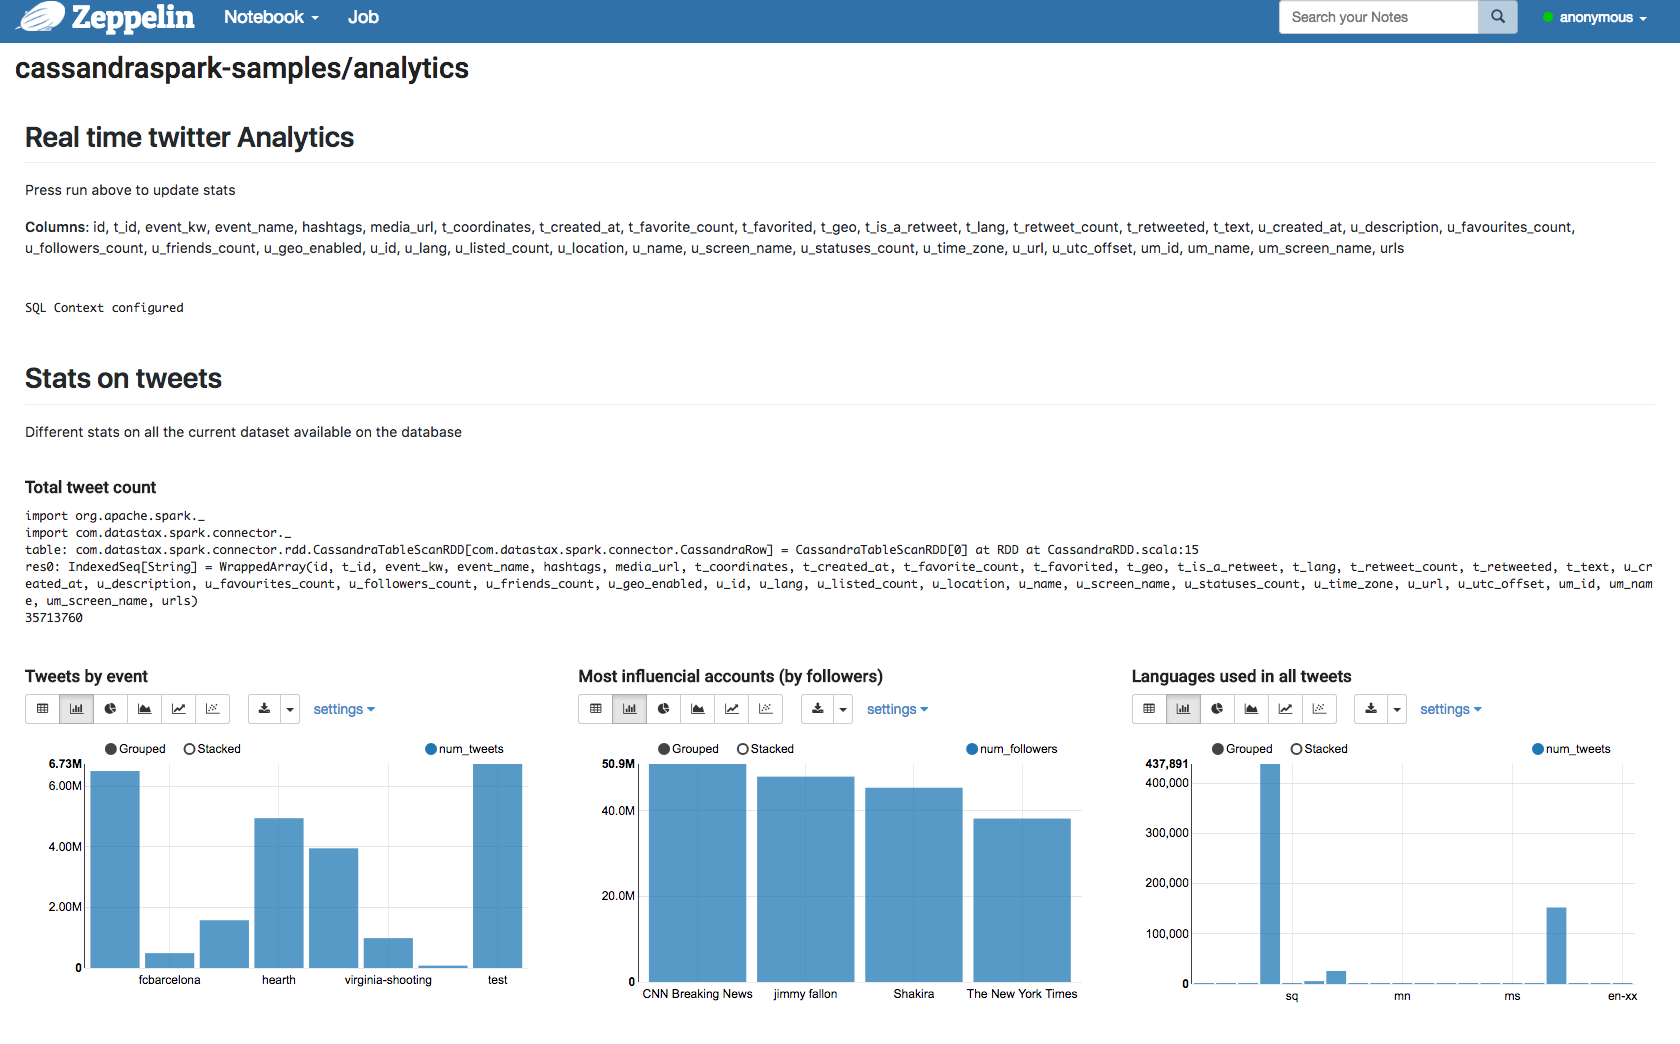
\includegraphics[width=\textwidth]{Figures/zeppelin}
\decoRule
\caption[Zeppelin visualization example]{Zeppelin server with some visualization from the dataset}
\label{fig:zeppelin}
\end{figure}

 % Chapter Template

\chapter{Evaluation} % Main chapter title

\label{Chapter6} % Change X to a consecutive number; for referencing this chapter elsewhere, use \ref{ChapterX}

In order to evaluate my work, I  compare the architecture and implementation of my prototype with the existing Project EPIC infrastructure along the dimensions of reliability, scalability, performance, and real time delivery.

\section{Reliability}

In order to evaluate my work, I  compare the architecture and implementation of my prototype with the existing Project EPIC infrastructure along the dimensions of reliability, scalability, performance, and real time delivery.

\subsection{Current infrastructure}

Reliability of the existing EPIC infrastructure needs to be studied separately across EPIC Collect and EPIC Analyze. EPIC Collect is designed to be highly available. It is implemented as a multi-threaded Java application; some threads are used to read the incoming tweet stream, some are used to classify tweets, and some are used to monitor the other threads. If the monitoring threads detect that one of the readers is no longer producing tweets for the classifiers, it can issue a command that causes the current connection to the Twitter Streaming API to be dropped and all of these threads to be deactivated. This action, in turn, causes another thread to detect that the Twitter connection is down and it then restarts the connection which causes readers, classifiers, and monitors to once again be instantiated. This approach can ensure reliable performance for many days; however, sometimes errors occur that cause all threads to lock up. To handle this situation, EPIC Collect makes use of a cron job that wakes up once per minute to examine the current length of the EPIC Collect log file. Each reader and classifier will send information to the log file and when data collection is proceeding smoothly, the log file is always increasing in size. As a result, if the cron job wakes up and discovers that the log file has not increased in size over the past minute, it assumes that the collection software has locked up. It will invoke a command to kill the previously running process and it then invokes the collection system, notes the size of the log file, and goes back to sleep. With these techniques, EPIC Collect has achieved 99\% uptime since the summer of 2012. The only problem that these techniques cannot account for is if the data center loses its network connection. When that happens, the cron job will be stuck in a cycle of terminating and restarting the software until the network connection is restored. Fortunately, complete loss of the data center’s connection to the Internet is a very rare event, happening only once in a four year period.

EPIC Analyze does not have the same level of reliability.In order for the web application to function, it requires that Redis and Solr be up and running. If these systems are not available, then the web application is non-functional. Compounding this situation is the fact that EPIC Analyze is deployed manually by its developers; there is no automated way to deploy it and there is no monitoring system detecting for system failure. As a result, there is also no automated recovery procedure. All aspects of the system deployment for EPIC Analyze require manual intervention by developers.


\subsection{System Prototype}

In the case of my system prototype, overall reliability is high, due to the use of a container orchestration system. Kubernetes provides two components to increase the reliability of our system. The first Kubernetes-provided component is the controller manager that runs on the master node of our cluster. This component is responsible for keeping track of all containers running on our cluster. It also follows the requests made by the infrastructure controller to ensure that the right number of replicas are created for the components that need them. For instance, in my prototype, I specify that there should 2 replicas of a Kafka broker available at all times. If any of those replicas go down, Kubernetes will detect that and launch a new one. This functionality extends to all of our containers; if any container stops running, the controller manager detects it and schedules a new instance of that container to run on an available node. This check is performed when the infrastructure controller makes new requests or when an existing node informs the controller manager that one of its containers went down.

The second Kubernetes-provided component is the scheduler. This component makes sure that new containers are scheduled on the best node possible. Kubernetes allows an engineer to configure the amount of memory and cpu permitted by a container; this information allows the scheduler to find the best fit for each deployment request.

With these two components, Kubernetes automates the deployment of containers on a cluster of machines and handles any failures automatically. Its services are significantly more advanced than the existing reliability measures put into place by the Project EPIC developers, who were more interested (at the time) in system functionality and not in automated failure recovery mechanisms beyond what was done to ensure reliable data collection.

Kubernetes provides one additional reliability-related feature and that is related to upgrading containers to provide new versions of the microservice within, it’s called rolling update. When performing an upgrade, the controller manager first deploys the new version of the component and ensures that it is up and running. It then removes the container containing the previous version of the component. I make use of this functionality with the Twitter Tracker component. When a new change to data collection is announced by the Event Manager UI component, the infrastructure controller arranges to have a new instance of the Twitter Tracker component deployed with the new state. It starts to collect tweets using the newly updated keyword list while the previous instance is still collecting data on the prior set of keywords. This approach ensures that no tweets are missed when the transition occurs. Twitter applications can only have one standing connection. When the new instance establishes a connection, Twitter will close the old connection ensuring that there won’t be any duplicated tweet stored in the transition.

Figure \ref{fig:pods} displays a typical report for the number of times the containers in our system prototype were restarted automatically by Kubernetes over a period of eleven days with no interaction from the user. The first thing to note is that all components remained active for the entire time period; that is data collection proceeded uninterrupted during those eleven days. However, due to system demands, Kubernetes may have found itself needing to, for instance, delete a container on an overloaded node and move it to a node that had more resources available. Given that my code is now fairly stable, if we increased the amount of memory on each node and added a few more nodes to our cluster, the total number of restarts would go down. But, given the limited resources I had during development, the more important issue is that despite limited resources, the system continued to run 24/7 with no interventions required by the developer.  Note: that in Figure \ref{fig:pods}, some instances are listed as only existing for two days; this discrepancy is due to the fact that Kubernetes will restart a container’s count if it needs to do a hard restart of the container. This occurs when Kubernetes issues a request for the container to shut down and it stays active, ignoring the request. This might occur due to the contained microservice crashing inside and thus unable to exit gracefully. As a result, Kubernetes is forced to kill the container without a graceful shutdown.



\begin{figure}
\centering
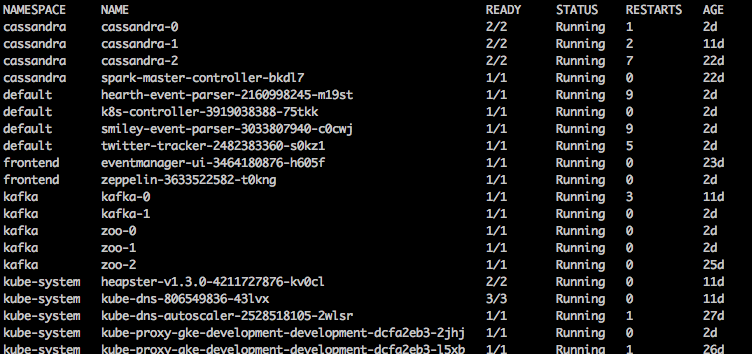
\includegraphics[width=\textwidth]{Figures/pods}
\decoRule
\caption[Kubernets restarts in eleven days]{Number of automated restarts by Kubernetes of the system prototype over a period of eleven days.}
\label{fig:pods}
\end{figure}

\section{Scalability}

The second dimension I am using for my evaluation is scalability. I am interested in how well both infrastructure deal with the ability to scale to large amounts of data. I want to avoid wasting system resources unnecessarily while having the capacity to scale and I want to understand how scaling impacts overall system performance.

\subsection{Current infrastructure}

Scalability with the existing infrastructure is not a straightforward process. With respect to throughput capacity, EPIC Collect would need a developer to manually launch a new instance with new Twitter credentials and set-up an a second cron job to monitor the second instance’s log files. That work is feasible but not straightforward and would have to be performed anew if more capacity was needed and a third instance was required. This situation is one reason why EPIC Collect does not perform data normalization; it simply classifies tweets with respect to the current set of events and then it stores them in Cassandra. If data normalization was added to the existing EPIC Collect then it would struggle to handle spikes in incoming traffic as it would not be able to automatically scale its capacity to handle demand.

With respect to storage capacity, EPIC Collect is in a better situation since it stores tweets to a four-node Cassandra cluster with terabytes of disk space available. If additional capacity is needed, a developer just needs to configure a new node and add it to the existing cluster. As with the discussion above concerning throughput capacity, while this works, it is hardly an automated approach to scaling the infrastructure on demand.
With respect to EPIC Analyze, the only component that is a target for scaling, apart from storage, is the frontend module that is currently written in Ruby on Rails. To do that, multiple instances of the application would need to be launched and a load balancer put in front of those instances. To make this work, the existing web application would need to be refactored such that session state can be made consistent across all of the instances. That is a straightforward engineering task but not simply by any means. Furthermore, maintaining a load balancer is a complex process when done manually and, as discussed above, all maintenance on EPIC Analyze has to be performed manually.

As a result, I must conclude that the existing Project EPIC infrastructure is not easy to scale.

\subsection{System Prototype}

Scaling my system prototype is much easier given the functionality gained from Kubernetes. When deploying a microservice via a container, I can specify how many replicas of that service I would like to deploy alongside it. The controller manager will try to schedule the requested number of replicas as long as there are enough system resources available across the cluster. Our ability to deploy multiple replicas is helped by the fact that most of our services were designed to be stateless. All of the state that they need to perform their task is contained in the messages that it receives. As a result, it doesn’t matter which replica handles a given input message. Replicas can also be automatically triggered based on CPU usage. If a container hits 90\% CPU utilization because it has experienced a spike in the number of input messages, Kubernetes can automatically spin up new replicas until the utilization goes down due to the fact that the new replicas can help the existing component handle the spike in messages.

While these services are largely automatic, a developer can always interact with Kubernetes directly to manually deploy additional components to help with scalability. The developer can issue these commands using the kubectl command line tool or via Kubernetes’s web interface.

Due to the features of container orchestration systems, my system prototype is much easier to scale than the existing Project EPIC infrastructure. 


\section{Performance}

I am unable to provide a comparison between the two infrastructures with respect to performance. Both systems have similar performance with respect to data collection but detailed tests and comparisons are not possible since EPIC Collect is a production system that other members of the Project EPIC team depend on for their research. As such, in this section, I provide insight into the performance my system prototype achieves on my small four-node cluster. As a reminder, each node in the cluster has access to one virtual CPU and four gigabytes of RAM. My test involves executing a Spark-based job on the cluster to count the number of words contained in all collected tweets. Each time I ran the query, the total number of tweets collected was different. I selected this particular test since word count is a highly parallelizable operation. It also demonstrates the integration of Spark into my system prototype.


The code entered into Zeppelin is shown in Listing \ref{lst:wordcount}.  The first line establishes a connection to Cassandra and creates a Spark Context object by which queries can be invoked. The second line expresses a series of transformations that Spark will apply to count all of the words of all tweets contained in Cassandra. It starts by selecting the text of the tweet, splitting the text into words, mapping each word into a pair (word, 1) and then reducing all such pairs by adding up the integers for each matching key. Thus all pairs like (cat, 1) would eventually turn into a single pair (cat, 1000) where 1000 represents the number of times that cat appears in the collected tweets. Finally, the pairs are inverted, e.g. (1000, cat), and then sorted in descending order.

The power of Spark is that all of these transformations are applied to every tweet in parallel and, furthermore, as much of the transformations are applied locally on every node before any data is sent to the master node for the final combination of pairs across nodes. Spark provides a mechanism to reveal how it will execute a query known as the debug string.



\begin{lstlisting}[language=scala, caption={WordCount Spark script},float, floatplacement=H, label={lst:wordcount}]
val table = sc.cassandraTable("twitter_analytics", "tweet")
val words = table.select("t_text").flatMap(l => l.getString("t_text").split(" "))
      .map(word => (word.toLowerCase,1)).reduceByKey(_ + _).map(_.swap).sortByKey(false,1)
\end{lstlisting}



Each indentation in the debug string is a map stage, and each + is a shuffle phase. As we can see in Listing \ref{lst:rddebug}, Spark delays shuffling data until it is time to execute the reduceByKey step. This makes sense since it can generate word pairs on each node without having to transfer data across nodes. However, once it needs to count the total number of words, it has to send data across nodes to a master node to create the final counts. It then performs one more shuffle when it sorts the final key-value pairs after swapping them from this format (cat, 1000) to this format (1000, cat).



\begin{lstlisting}[language=scala, caption={Debug string rdd}, float, floatplacement=H, label={lst:rddebug}]
(1) ShuffledRDD[112] at sortByKey at <console>:31 []
+-(176) MapPartitionsRDD[111] at map at <console>:31 []
    |   ShuffledRDD[110] at reduceByKey at <console>:31 []
    +-(176) MapPartitionsRDD[109] at map at <console>:31 []
        |   MapPartitionsRDD[108] at flatMap at <console>:31 []
        |   CassandraTableScanRDD[107] at RDD at CassandraRDD.scala:15 []
\end{lstlisting}

As we can see in Figure \ref{fig:wordcountplot},  the word count performance is not linear but, indeed,  performs better with larger numbers of tweets to analyze (see the increase in tweets processed per second in Table \ref{tab:numtweets}). The likely reason for this performance curve is that there is a certain amount of overhead that is incurred each time to stage the job and perform the shuffle steps at the end, counting up the pairs and sorting them. However, as the number of tweets increases, each individual node can do more work uninterrupted and can execute as quickly as possible without the need for coordination messages. As a result, the performance increases and keeps the overall time sublinear at least for datasets in the millions of tweets.


\begin{figure}
\centering
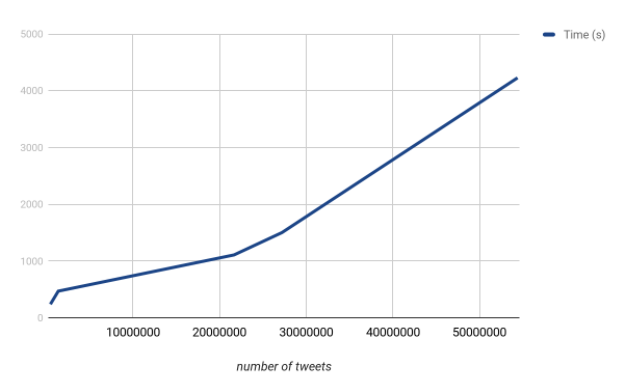
\includegraphics[width=\textwidth]{Figures/wordcountplot}
\decoRule
\caption[Wordcount time plot]{Plot on wordcount time for dataset size}
\label{fig:wordcountplot}
\end{figure}


\begin{table}
\centering
\begin{tabular}{l l}
\toprule
\textbf{Number of tweets} & \textbf{Time (s)} \\
\midrule
490199 & 238 \\
1400884 & 469 \\
21680851 & 1107 \\
27199614 & 1500 \\
54395957 & 4228 \\
\bottomrule\\
\end{tabular}

\caption{Number of tweets in dataset vs seconds took to perform word count}
\label{tab:numtweets}
\end{table}


\section{Software development and maintenance: Ken start here}

One of our goals was to develop a system that was easier to maintain. That was one of the reasons to adapt microservices was to avoid having components get outdated by making it easier for developers to onboard on the code and maintain it. In addition we also want to compare how easy would be to replace a component and code it from the ground up.

\subsection{Current infrastructure}

Currently the code is divided in 2 big monoliths. This can be a disadvantage on terms that developers must dig into the code of at least one of them in order to perform maintenance. This can be an small overhead as both of the projects are quite big. 

EPIC Analyze has 5086 lines of code. On boarding this part can be difficult. Specially since it uses a pretty closed framework as Ruby on Rails is. This can be a difficulty in terms of having to write new code, anyone who wants to write something need to learn the usage of Ruby on Rails. This framework is big and has a quite fast learning curve. However, it can be difficult as it implements practices that sometimes are not obvious for a developer coming from other frameworks. In addition to the code, we have a slow deployment process. In order to update the deployed version of EPIC Analyze, we need to restart the server manually. This makes it difficult to deploy, which in result turns into a really slow development process. Development for Analyze happens on a git repository, this makes collaboration easier between different developers.

EPIC Collect is difficult to analyze as it’s not on a git repository. Written in Java it’s built thinking on efficiency first.  This can be a bit of a difficulty in terms of collaborating and maintaining the code. In addition deploying new versions involves a lot of effort as it doesn’t only involve deploying the code, but also maintain the Tomcat server. We also need to take into account all the processes that are keeping EPIC Collect alive. Due to the fact that this scripts are embedded onto the development of EPIC Collect, we need to redeploy them manually.

\subsection{Proposed infrastructure}

The proposed infrastructure is divided into multiple different pieces. On one side we have the components code, divided between Python and Go code. On the other side we have the declaratives documents on YAML that specify how to deploy the infrastructure into Kubernetes.

\begin{itemize}
	\item \textit{Twitter tracker (Go)}: 108 lines 
	\item \textit{Kubernetes controller (Python)}: 145 lines
	\item \textit{Event manager UI (Python/Django)}: 2090 lines
	\item \textit{Tweet normalizer (Python)}: 209 lines
\end{itemize}

Code is more equilibrated distributed between different parts. The good thing is that we are not tied into an specific and unique framework. Making code small makes it easier for other developers to understand the purpose of each component. In addition thanks to separating responsibilities into microservices we can make collaboration easier by letting different developers work on different parts without crossing each other.

Something that also helps is that we can use different technologies in each component. This means that we can focus on building on the best available option for what we need to do. It also allows for a better pivoting of a component into a language that the maintainer prefers. If it can be containerized then it doesn’t matter what language or technology stack we use. It will be easily deployed into Kubernetes.

Finally we have the YAML files that store how the Kubernetes system looks like. All the system is declared in 3345 lines. There are many tools being released that will help make this code smaller. However right now the best option is to manually write and review each component in Kubernetes YAML files.



% Chapter Template

\chapter{Future Work} % Main chapter title

\label{Chapter7} % Change X to a consecutive number; for referencing this chapter elsewhere, use \ref{ChapterX}

This project was focused on proving the advantages that moving a Big data Analytics system to a container orchestration system could bring. Therefore the project itself would be more defined as a proof of concept than a production ready product. In that direction then is where future work could be focused on. The system can be improved to make it more production ready. Some feature that can be improved in this sense is a better study on each component resource usage. This could be used to make sure that each component is deployed with the corresponding resource usage. 

Another feature that would need to be added into this before deploying is a centralized system for authentication and authorization. The proposed system doesn’t have any security on purpose, we wanted to prove how the system would perform, so there was no need to make security a priority. In that way, developing and adapting the frontend components to use a centralized authorization protocol like JWT within a centralized microservice. This is not an easy part, especially since some of the system parts like Spark are using shared resources to work. Administering resource usage between users is a really important work.

Cassandra tables would need to be optimized for the system usage as well. For this project we used a really naive approach to tweet storage. It works pretty great for what we needed to do. However, if we want to replace the current system, this would need to be improved. A way to make this better is by upgrading event\_name to partition key as described previously. In addition we would need to add logic in the partition assignment for the tweet normalizer, as Cassandra limits the amount of row a partition can contain and we need a way to make it easier for data to be distributed between all nodes in the best way. We could do this by assigning a random partition number when the tweet normalizer starts and choose a new value every 100.000 stored tweets. This would need to be studied more carefully in the future.

Then on the other side, thanks to the system extensibility, there are a few directions that the system could be improved. For example, we could add a real-time query resolver for a very specific query by plugging it into the raw\_tweets queue and make it analyze the data. Or we could add other systems for specific queries like Elastic search for word search or text analysis. In addition we could extend the system to include better collaboration tools like a notification system plugged into the event\_updates queue. The possibilities are quite a lot, the best part is that this doesn’t need to upgrade other components of the system at any time.

% Chapter Template

\chapter{Related Work} % Main chapter title

\label{Chapter8} % Change X to a consecutive number; for referencing this chapter elsewhere, use \ref{ChapterX}

There has been a lot of research on big data analytics. Open source tools like Hadoop and Spark have made available scalable, distributed computation to the general public. In addition, thanks to the progress in big data storage, with systems like Cassandra, hosting internal storage has never been easier. However there is not a lot of work regarding using container-orchestration for big data analysis systems. There has been a lot work in both fields, but there is not a lot of work about combining them.

The work presented by \parencite{smack} is probably the closest approach to the system I present here. The main differences are in the actor system and the orchestration platform. Instead of using Mesos for orchestration and Akka for actors, I preferred to use Kubernetes with container microservices instead of actors. The stack described also uses Spark Streaming to deploy a Lambda architecture which could be done in the current infrastructure extending the capabilities of the system. The main reason for avoiding Spark Streaming has been that its micro batching focus could involve losing tweets during the normalization process. Furthermore, the reason to avoid Akka for actors was that it had similar features to Kafka and microservices in Kubernetes. In that way, I considered that adding Akka would make the system more complex and therefore more difficult to maintain.

There has also been previous work trying to approach big data analytics to a higher scalability like this paper from 2014 \parencite{scalableHadoop}. This system proposal is agnostic on how to deploy such systems, leaving the developer to deal with it. As container and container orchestrated systems were not popular at that time, they are not considered. Its main approach to getting these systems to scale is via the use of different Hadoop components. Currently, Spark is preferred over Hadoop, given the increased performance made possible via its memory-based approch to MapReduce.

In \parencite{lambda2014}, we see a similar approach using Hadoop and Pig in the batch layer instead of Cassandra and Spark. They also incorporate a streaming layer for real-time analysis making use of the lambda infrastructure. In \parencite{streamingAnalysis}, we can see Zeppelin used as a dashboard interface similar to our work. However none of this systems made use of the container-orchestrated approach and so lack the scalability and reliablity benefits that they provide.

% Chapter Template

\chapter{Future Work} % Main chapter title

\label{Chapter9} % Change X to a consecutive number; for referencing this chapter elsewhere, use \ref{ChapterX}

This project was focused on demonstrating the advantages achieved by migrating a big data analytics system to a container-orchestration system. My system prototype has an impressive set of features but it is, however, just a proof of concept. As such, there are many areas for improvement including resource usage, security, database optimization, and extensibility.

With respect to resource usage, there is room for improvement on understanding the usage constraints of each of my system components. If I could identify upper and lower bounds for each component, I could provide the Kubernetes scheduler with even more information in which to make optimization decisions and container allocations.

Another feature that is needed is a centralized system for authentication and authorization. My research prototype deliberatly avoided imposing any security measures as our focus was on what was feasible with respect to reliablity and scalability. However, if this system were to be transitioned into a production environment, then a wide variety of security-related techniques would need to be adopted: encryption of data, securing of individual components, the addition of user and system roles and authorization of those roles to access particular types of data and engage in particular types of operations.

There is plenty of room for improvement with respect to the structure of my Cassandra tables. For my thesis work, I used a  naive approach to tweet storage. It works well for what I needed to do but there are plenty of ways in which it could be improved. A way to make this better is by upgrading event\_name to be a partition key. This would allow Cassandra to cluster tweets that belong to the same event improving all queries that are event-based. In addition, I would need to add logic in the partition assignment for the tweet normalizer, as Cassandra limits the amount of rows a partition can contain and we need a way to make it easier for data to be distributed across all nodes. We could do this by assigning a random partition number when the tweet normalizer starts and choose a new value every one hundred thousand stored tweets. This would need to be studied more carefully in the future.

With respect to system extensibility, there are a few ways that the prototype could be improved. For example, I could add a real-time query resolver for a very specific query by plugging it into the raw\_tweets queue and make it analyze the data. Or I could add other systems for specific queries like Elastic search for full-text search or analysis. In addition we could extend the system to include better collaboration tools like a notification system plugged into the event\_updates queue.

As one can see, there are many possibilities for improvement and due to the benefits of container-orchestration system, many of these improvements can be done in isolation without the need to upgrade all of the components at once.

% Chapter Template

\chapter{Conclusions} % Main chapter title

\label{Chapter10} % Change X to a consecutive number; for referencing this chapter elsewhere, use \ref{ChapterX}

Container orchestrated technologies make it easier to develop Big Data Analytics systems. Their abstraction layer allows for a separation of responsabilities between developers and system operators, allowing them to work without overlapping their work. This opens a gate for innovation on the Big Data Analytics field, as improvements can be developed separately for infrastructure and software. It also opens a gate to new approaches to system state, extracting the state into the ruling container orchestrated system.

In our case, using container orchestration to recreate Project EPIC infrastructure has proved to be easier to scale. It also, has kept reliance from the previous system, abstracting it and making it part of the orchestration system. It has proved to be an easier to mantain infrastructure, as components are smaller and it's easier to make a more continous development and deployment cycle. In addition, container systems like Docker allows for developers to focus more on the application logic instead of worrying about deployment infrastructure. Finally, container orchestrated systems allows for a better reliance by managing the deployment cycle and ensuring a certain amount of deployed instance at any point.

In conclusion, we have proved that container orchestration systems can become a great option when developing Big Data Analytics infrastructures that require a flexible scaling and high reliability. However there are still some limitations. Will we see this approach become a standard the facto? Or will container orchestrated systems only succeed in transactional infrastructures?

% \section{Software development in microservices architectures}

% Thanks to container-orchestrated systems and the popularization of container systems, software development is easier. With microservices, focus moves out of one component software architecture to organizing the whole system. Now, we can focus on packaging alone components instead of having to packaging all of them at once, which makes the development more flexible. This would allow for a more continuous development in the system allowing for a better performance optimization, and an easier way to keep the system updated with the last set of technologies.


%----------------------------------------------------------------------------------------
%	THESIS CONTENT - APPENDICES
%----------------------------------------------------------------------------------------

\appendix % Cue to tell LaTeX that the following "chapters" are Appendices

% Include the appendices of the thesis as separate files from the Appendices folder
% Uncomment the lines as you write the Appendices

% Appendix A

\chapter{Microservices code} % Main appendix title

\label{AppendixA} % For referencing this appendix elsewhere, use \ref{AppendixA}

Attached here is a version of the code developed for some of the custom microservices discussed in \autoref{Chapter4}. The event manager UI is not included due to the extensivity of the codebase.

\section{Twitter Tracker}

\subsection{twitter\_tracker.go}

\begin{lstlisting}[language=Golang]
package main

// OAuth1
import (
	"github.com/dghubble/oauth1"
	"os"
	"bufio"
	"strings"
	"net/url"
	"gopkg.in/Shopify/sarama.v1"
	"log"
)

// Line separator function, detects new lines
func scanLines(data []byte, atEOF bool) (advance int, token []byte, err error) {
	if atEOF && len(data) == 0 {
		return 0, nil, nil
	}
	if i := strings.Index(string(data), "\r\n"); i >= 0 {
		// We have a full '\r\n' terminated line.
		return i + 2, data[0:i], nil
	}
	// If we're at EOF, we have a final, non-terminated line. Return it.
	if atEOF {
		return len(data), dropCR(data), nil
	}
	// Request more data.
	return 0, nil, nil
}

func dropCR(data []byte) []byte {
	if len(data) > 0 && data[len(data)-1] == '\n' {
		return data[0: len(data)-1]
	}
	return data
}


func main() {
	// Get environment variables
	var access_token = os.Getenv("ACCESS_TOKEN")
	var token_secret = os.Getenv("ACCESS_TOKEN_SECRET")
	var consumer_key = os.Getenv("CONSUMER_KEY")
	var consumer_secret = os.Getenv("CONSUMER_SECRET")
	var tokens = os.Getenv("TOKENS")
	var kafka_servers = strings.Split(os.Getenv("KAFKA_SERVERS"),",")

	// Prepare OAuth1 client
	conf := oauth1.NewConfig(consumer_key, consumer_secret)
	token := oauth1.NewToken(access_token, token_secret)
	client := conf.Client(oauth1.NoContext, token)
	v := url.Values{}
	v.Set("track", tokens)

	// Get url for stream
	stream_url := "https://stream.twitter.com/1.1/statuses/filter.json?" + v.Encode()

	// Connect to URL with POST
	resp, err := client.Post(stream_url, "application/json", nil)

	if err != nil {
		log.Fatalf("Error while connecting to twitter: %s", err)
		panic(err)
		return
	}

	if resp.StatusCode != 200 {
		log.Fatalf("Error while connecting to twitter, status code returned: %d", resp.StatusCode)
		panic(err)
		return
	}

	// Create buffer scanner for request and split by custom function
	scanner := bufio.NewScanner(resp.Body)
	scanner.Split(scanLines)

	// Start asyncronous kafka producer
	producer, err := sarama.NewAsyncProducer(kafka_servers, nil)

	// Close producer before exiting program
	defer func() {
		if err := producer.Close(); err != nil {
			log.Fatalln(err)
		}
	}()

	if err != nil {
		log.Fatalf("Error while bootstraping Kafka producer: %s", err)
		panic(err)
		return
	}

	// Start separate thread to track Kafka produced errors
	go func() {
		for err := range producer.Errors() {
			log.Fatalf("Kafka error: %s", err)
			// Exit application if any error from Kafka
			// Force Kubernetes to recover
			os.Exit(2)
		}
	}()

	// Main loop to scan request. Only breaks if error from Kafka.
	for scanner.Scan() {
		tweet := scanner.Bytes()
		if len(token) == 0 {
			// empty keep-alive
			continue
		}

		// Send tweet to producer
		producer.Input() <- &sarama.ProducerMessage{Topic: "raw_tweets", Key: nil, Value: sarama.StringEncoder(tweet)}
		log.Printf("Tweet received")
	}
	log.Printf("Closing")

}
\end{lstlisting}
\newpage
\section{Twitter Normalizer}

\subsection{model.py}

\begin{lstlisting}[language=Python]
# -*- coding: utf-8 -*-
from __future__ import unicode_literals
import logging
import os
import socket
import uuid
from datetime import datetime
import ujson
from cassandra.cluster import Cluster
from cassandra.cqlengine import columns, connection
from cassandra.cqlengine.management import sync_table
from cassandra.cqlengine.models import Model

CASSANDRA_IPS = list(
    map(socket.gethostbyname, os.environ.get('CASSANDRA_NODES', '127.0.0.1').replace(' ', '').split(',')))
KEYSPACE = 'twitter_analytics'

# Tweet model definition as Python Class
class Tweet(Model):
    id = columns.UUID(primary_key=True, default=uuid.uuid4)
    event_name = columns.Text(index=True)
    t_id = columns.Text(primary_key=True, clustering_order="DESC")
    event_kw = columns.Text()
    t_created_at = columns.DateTime()
    t_text = columns.Text()
    t_retweet_count = columns.Integer()
    t_favorite_count = columns.Integer()
    t_geo = columns.Text()
    t_coordinates = columns.Text()
    t_favorited = columns.Boolean()
    t_retweeted = columns.Boolean()
    t_is_a_retweet = columns.Boolean()
    t_lang = columns.Text()
    u_id = columns.Text()
    u_name = columns.Text()
    u_screen_name = columns.Text()
    u_location = columns.Text()
    u_url = columns.Text()
    u_lang = columns.Text()
    u_description = columns.Text()
    u_time_zone = columns.Text()
    u_geo_enabled = columns.Boolean()
    media_url = columns.Text()
    um_screen_name = columns.Text()
    um_name = columns.Text()
    um_id = columns.Text()
    u_followers_count = columns.Integer()
    u_friends_count = columns.Integer()
    u_listed_count = columns.Integer()
    u_favourites_count = columns.Integer()
    u_utc_offset = columns.Integer()
    u_statuses_count = columns.Integer()
    u_created_at = columns.DateTime()
    hashtags = columns.List(value_type=columns.Text)
    urls = columns.List(value_type=columns.Text)


logging.info('Connecting to cassandra...')

cluster = Cluster(CASSANDRA_IPS)
with cluster.connect() as session:
    logging.info('Creating keyspace...')
    # Keyspace creation
    session.execute("""
           CREATE KEYSPACE IF NOT EXISTS %s
           WITH replication = { 'class': 'SimpleStrategy', 'replication_factor': '1' }
           """ % KEYSPACE)

    # Establish connection with Cassandra cluster
    connection.setup(CASSANDRA_IPS, KEYSPACE, protocol_version=3)

    #Table creation
    logging.info('Creating table...')
    sync_table(Tweet)


def create_dict(event_key, event_kw, tweet):
    return {
        'id':str(uuid.uuid1()),
        't_id': tweet['id_str'],
        'event_kw': ','.join(event_kw),
        'event_name': event_key,
        't_created_at': datetime.strptime(tweet['created_at'], '%a %b %d %H:%M:%S +0000 %Y').isoformat(),
        't_text': tweet['text'],
        't_retweet_count': tweet['retweet_count'],
        't_favorite_count': tweet['favorite_count'],
        't_geo': str(tweet['geo']),
        't_coordinates': str(tweet['coordinates']),
        't_favorited': tweet['favorited'],
        't_retweeted': tweet['retweeted'],
        't_is_a_retweet': 'retweeted_status' in tweet,
        't_lang': tweet['lang'],
        'u_id': tweet['user']['id_str'],
        'u_name': tweet['user']['name'],
        'u_screen_name': tweet['user']['screen_name'],
        'u_location': tweet['user']['location'],
        'u_url': tweet['user']['url'],
        'u_lang': tweet['user']['lang'],
        'u_description': tweet['user']['description'],
        'u_time_zone': tweet['user']['time_zone'],
        'u_geo_enabled': bool(tweet['user']['geo_enabled']),
        'u_followers_count': tweet['user']['followers_count'],
        'u_friends_count': tweet['user']['friends_count'],
        'u_favourites_count': tweet['user']['favourites_count'],
        'u_statuses_count': tweet['user']['statuses_count'],
        'u_created_at': datetime.strptime(tweet['user']['created_at'], '%a %b %d %H:%M:%S +0000 %Y').isoformat(),
        'hashtags': list(map(lambda h: h['text'], tweet['entities']['hashtags'])),
        'urls': list(map(lambda url: url['url'], tweet['entities']['urls'])),
        # Concat names with a space separation
        'um_screen_name': ' '.join(map(lambda um: str(um['screen_name']), tweet['entities']['user_mentions'])),
        'um_name': ' '.join(map(lambda um: str(um['name']), tweet['entities']['user_mentions'])),
        'um_id': ' '.join(map(lambda um: str(um['id_str']), tweet['entities']['user_mentions'])),
        'media_url': ' '.join(map(lambda m: str(m['media_url_https']), tweet['entities']['media']))
        if 'media' in tweet['entities'] else None,

    }


session = connection.session
prep_query = session.prepare("INSERT INTO %s.tweet JSON ?" % KEYSPACE)


def save_tweet(tweet, event_key, event_kw):
    session.execute_async(prep_query, [ujson.dumps(create_dict(event_key, event_kw, tweet)), ])
\end{lstlisting}

\newpage


\subsection{tweetparser.py}


\begin{lstlisting}[language=Python]
import logging
import os
import sys
import ujson
from confluent_kafka import Consumer, KafkaError, KafkaException

EVENT_KEY = os.environ.get('EVENT_KEY', '')
assert EVENT_KEY, 'Event key must be specified as environment variable'

TOKENS = list(filter(None, os.environ.get('TOKENS', '').split(',')))
assert TOKENS, 'Tokens can\'t be empty'

KAFKA_SERVER = os.environ.get('KAFKA_SERVERS', 'localhost:9092')

def main(save):
    conf = {'bootstrap.servers': KAFKA_SERVER,
            'group.id': EVENT_KEY,
            'session.timeout.ms': 6000,
            'default.topic.config': {'auto.offset.reset': 'smallest'}
            }
    # Create Kafka consumer with specified configuration
    c = Consumer(**conf)

    # Custom function for assignment printing
    def print_assignment(consumer, partitions):
        logging.info('Assignment: %s' % partitions)

    # Subscribe to topics
    c.subscribe(['raw_tweets', ], on_assign=print_assignment)

    msg_count = 0
    while True:
        msg = c.poll()
        if msg is None:
            continue
        if msg.error():
            # Error or event
            if msg.error().code() == KafkaError._PARTITION_EOF:
                # End of partition event
                logging.info('%% %s [%d] reached end at offset %d' % (msg.topic(), msg.partition(), msg.offset()))
            elif msg.error():
                # Error
                raise KafkaException(msg.error())
        else:
            tweet = None
            try:
                tweet = ujson.loads(msg.value())
            except TypeError:
                logging.error("Message not json: %s" % msg.value())
                continue
            except ValueError:
                logging.error("Message not json: %s" % msg.value())
                continue

            # Twitter internal messages are discarded here
            if 'text' not in tweet:
                logging.info('Internal message: %s' % tweet)
                continue
            msg_count += 1

            # Check if tweet should be stored
            if any(token in tweet['text'] for token in TOKENS):
                logging.info('Tweet accepted: %s:%d:%d: key=%s tweet_id=%s' %
                             (msg.topic(), msg.partition(), msg.offset(),
                              str(msg.key()), tweet['id']))
                save(tweet, EVENT_KEY, TOKENS)

        # Readiness write on first message (used by Kubernetes)
        if msg_count == 1:
            open('/tmp/healthy', 'a').close()


if __name__ == "__main__":
    logging.basicConfig(
        format='%(asctime)s.%(msecs)s%(levelname)s:%(message)s',
        level=logging.INFO
    )
    import model

    logging.info('Event: %s' % EVENT_KEY)
    logging.info('Tracking keywords: %s' % ','.join(TOKENS))
    logging.info('Kafka servers: %s' % KAFKA_SERVER)
    logging.info('Connecting to Cassandra...')
    logging.info('Start stream track')
    if not TOKENS:
        logging.error('Tokens can\'t be empty')
    main(model.save_tweet)

\end{lstlisting}
\newpage
\section{Infrastructure Controller}

There's also YAML templates to generate the deployments that are sent to Kubernetes. I don't include them here. To check some sample YAML file see \autoref{AppendixB}

\subsection{start.py}

\begin{lstlisting}[language=Python]
import json
import logging
import os

from kafka import KafkaConsumer

import k8scontroller

bootstrap_servers = os.environ.get('KAFKA_SERVERS', 'localhost:9092').split(',')
topic = os.environ.get('KAFKA_TOPIC', 'events')

TEST_TYPE = 'test'
EVENT_TYPE = 'event'
QUERIES_TYPE = 'queries'

UPDATE_ACTION = 'update'
REFRESH_ACTION = 'refresh'
IGNORE_ACTION = 'ignore'


def main():
    consumer = KafkaConsumer(topic, group_id='k8scontroller-eventparser', bootstrap_servers=bootstrap_servers,
                             value_deserializer=lambda m: json.loads(m.decode('utf-8')))

    for message in consumer:
        value = message.value
        type_ = value['type']
        action = value['action']
        if (action == UPDATE_ACTION or action == REFRESH_ACTION) and type_ == EVENT_TYPE:
            data = value['data']
            try:
                if data['tracking'] and data['tokens'].replace(' ', '').replace(',', ''):
                    k8scontroller.apply_eventparser(data['code'], data['tokens'])
                    logging.info('Created event partser for event: %s' % data['code'])
            except KeyError:
                logging.info('Message received was not formatted correctly. Message:\n %s' % data)
        elif (action == UPDATE_ACTION or action == REFRESH_ACTION) and type_ == QUERIES_TYPE:
            tokens = value['data']
            try:
                k8scontroller.update_queries(tokens)
                logging.info('Updated twitter streaming with queries: %s' % tokens)
            except KeyError:
                logging.info('Message received was not formatted correctly. Message:\n %s' % value)


if __name__ == "__main__":
    logging.basicConfig(
        format='%(asctime)s.%(msecs)s:%(name)s:%(thread)d:%(levelname)s:%(process)d:%(message)s',
        level=logging.INFO
    )
    logging.info('Checking Kubernetes connection...')
    logging.info('Kubernetes current pods ips: %s' % k8scontroller.get_pod_ips())

    logging.info('Kafka servers: %s' % ','.join(bootstrap_servers))
    logging.info('Start tracking changes')
    main()
\end{lstlisting}

\newpage
\subsection{k8scontroller.py}

\begin{lstlisting}[language=Python]
import os

import logging
import yaml
from kubernetes import client, config
from kubernetes.client.rest import ApiException

KAFKA_SERVERS = os.environ.get('KAFKA_SERVERS', 'localhost:9092')
CASSANDRA_SERVERS = os.environ.get('CASSANDRA_SERVERS', 'localhost')

ACCESS_TOKEN = os.environ.get("ACCESS_TOKEN", "ENTER YOUR ACCESS TOKEN")
ACCESS_TOKEN_SECRET = os.environ.get("ACCESS_TOKEN_SECRET", "ENTER YOUR ACCESS TOKEN SECRET")
CONSUMER_KEY = os.environ.get("CONSUMER_KEY", "ENTER YOUR API KEY")
CONSUMER_SECRET = os.environ.get("CONSUMER_SECRET", "ENTER YOUR API SECRET")
TWEET_CASSANDRA_VERSION = os.environ.get("TWEET_CASSANDRA_VERSION", "1.2.1")
TWITTER_STREAMING_VERSION = os.environ.get("TWITTER_STREAMING_VERSION", "1.1.0")


def load_config():
    try:
        config.load_kube_config()
    except:
        config.load_incluster_config()


def get_pod_ips():
    # Configs can be set in Configuration class directly or using helper utility

    load_config()

    v1 = client.CoreV1Api()
    logging.info("Listing pods with their IPs:")
    ret = v1.list_pod_for_all_namespaces(watch=False)
    return list(map(lambda x: x.status.pod_ip, ret.items))


def apply_eventparser(event_code, keywords):
    load_config()

    with open("k8sdeployments/tweet_cassandra.yaml") as f:
        name = '%s-event-parser' % event_code
        dep = yaml.load(
            f.read()
                .replace('{{code}}', event_code)
                .replace('{{keywords}}', keywords)
                .replace('{{name}}', name)
                .replace('{{version}}', TWEET_CASSANDRA_VERSION)
                .replace('{{kafka-servers}}', KAFKA_SERVERS)
                .replace('{{cassandra-servers}}', CASSANDRA_SERVERS)



        )

        k8s_beta = client.ExtensionsV1beta1Api()
        try:
            resp = k8s_beta.create_namespaced_deployment(
                body=dep, namespace="default")
        except ApiException as e:
            resp = k8s_beta.patch_namespaced_deployment(name,
                                                        body=dep, namespace="default")

        return resp


def update_queries(queries):
    load_config()
    with open("k8sdeployments/twitter_tracker.yaml") as f:
        name = 'twitter-tracker'
        dep = yaml.load(
            f.read()
                .replace('{{a_token}}', ACCESS_TOKEN)
                .replace('{{a_token_secret}}', ACCESS_TOKEN_SECRET)
                .replace('{{c_key}}', CONSUMER_KEY)
                .replace('{{c_secret}}', CONSUMER_SECRET)
                .replace('{{queries}}', ','.join(queries))
                .replace('{{version}}', TWITTER_STREAMING_VERSION)
                .replace('{{kafka-servers}}', KAFKA_SERVERS)
        )

        k8s_beta = client.ExtensionsV1beta1Api()
        try:
            resp = k8s_beta.create_namespaced_deployment(
                body=dep, namespace="default")
        except ApiException as e:
            resp = k8s_beta.patch_namespaced_deployment(name,
                                                        body=dep, namespace="default")

        return resp
\end{lstlisting}



% Appendix Template

\chapter{Kubernetes YAML configuration} % Main appendix title

\label{AppendixB} % Change X to a consecutive letter; for referencing this appendix elsewhere, use \ref{AppendixX}

As we stated in \autoref{Chapter6}, all the system has been built using Kubernets YAML configuration files. Here is an example for the Event Manager UI deployment.

\section{Event Manager UI deployment file}

\begin{lstlisting}[]
apiVersion: extensions/v1beta1
kind: Deployment
metadata:
  name: k8s-controller
spec:
  replicas: 1
  template:
    metadata:
      labels:
        app: k8s-controller
    spec:
      terminationGracePeriodSeconds: 10
      containers:
      - name: k8scontroller
        image: projectepic/k8s-controller:latest
        resources:
          limits:
           memory: 50Mi
           cpu: "50m"
          requests:
           memory: 50Mi
           cpu: "50m"
        env:
            - name: KAFKA_SERVERS
              value: kafka-0.broker.kafka.svc.cluster.local:9092,kafka-1.broker.kafka.svc.cluster.local:9092,kafka-2.broker.kafka.svc.cluster.local:9092
            - name: CASSANDRA_SERVERS
              value: cassandra-0.cassandra.cassandra.svc.cluster.local,cassandra-1.cassandra.cassandra.svc.cluster.local
            - name: ACCESS_TOKEN
              valueFrom:
                secretKeyRef:
                  name: twsecret
                  key: access_token
            - name: ACCESS_TOKEN_SECRET
              valueFrom:
                secretKeyRef:
                  name: twsecret
                  key: access_token_secret
            - name: CONSUMER_KEY
              valueFrom:
                secretKeyRef:
                  name: twsecret
                  key: consumer_key
            - name: CONSUMER_SECRET
              valueFrom:
                secretKeyRef:
                  name: twsecret
                  key: consumer_secret
            - name: TWEET_CASSANDRA_VERSION
              value: 1.2.7
            - name: TWITTER_STREAMING_VERSION
              value: 1.0.4
\end{lstlisting}


%\include{Appendices/AppendixC}

%----------------------------------------------------------------------------------------
%	BIBLIOGRAPHY
%----------------------------------------------------------------------------------------

\printbibliography[heading=bibintoc]

%----------------------------------------------------------------------------------------

\end{document}
